\chapter{Le plateau et son implémentation}
Le plateau du jeu des amazones est un échiquier classique. L'utilisation d'un graphe via une matrice d'adjacence, représentant les liaisons entre les différentes cases de cet échiquier, était imposée. 

L'utilisation seule du graphe peut être contraignante. En effet, lors de la partie, le plateau change de disposition au fur et à mesure que les joueurs jouent. Cela implique alors de modifier à chaque coup l'état du graphe, qui demanderait plusieurs opérations contraignantes. C'est pour cela qu'il a été décidé que le graphe soit et reste statique. L'introduction d'un monde via la création d'une structure permettrait une mise à jour plus facile et moins coûteuse du plateau de jeu.  
\section{Représentation du monde}

Pour ce faire, une structure \texttt{world\_t} a été implémentée afin d'enregistrer l'évolution du monde au cours de la partie. Cette structure contient un entier représentant la largeur du plateau, et un pointeur de type \texttt{enum sort} permettant de créer le plateau. Cette énumération permet de distinguer les différents états d'une case, en effet, elle peut être :
\begin{itemize}
    \item libre,
    \item bloquée par une tour blanche,
    \item bloquée par une tour noire,
    \item bloquée par une flèche.
\end{itemize}

\bigbreak

L'utilisation seule d'un pointeur aurait déjà permis de renvoyer le monde à la sortie des différentes fonctions agissant dessus. De plus, en utilisant les allocations dynamiques, cela évite des erreurs de mémoire sur la pile, plus difficiles à identifier avec valgrind.

Cependant, pour aider à l'initialisation et à la libération de cette allocation dynamique, ce pointeur a été couplé avec la largeur du monde dans la structure \texttt{world\_t}, rendant le monde plus malléable, et permettant d'afficher de façon claire le plateau de jeu.

De plus, le tableau est alloué dynamiquement en fonction de la taille du monde. Ce qui permet de réduire l'espace mémoire occupé par la structure. Les cases étant ordonnées, un simple parcours associant les états de chaque case à un caractère permet un affichage simple de la partie en cours, comme présenté en figure \ref{fig:affichage_partie}. 

\medbreak

\begin{figure}[H]
    \centering
    \begin{subfigure}{0.4\textwidth}
        \centering
        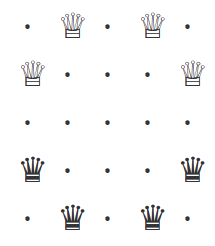
\includegraphics[scale=0.4]{log_0.png}
        \caption{État initial.}
        \label{subfig:affichage_etat_initial}
    \end{subfigure}
    \begin{subfigure}{0.52\textwidth}
        \centering
        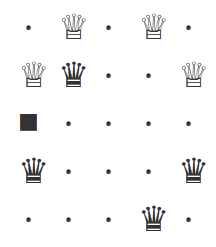
\includegraphics[scale=0.4]{log_1.png}
        \caption{1er coup du joueur noir.}
        \label{subfig:affichage_premier_coup}
    \end{subfigure}
    \caption{Affichage du monde, à l'état initial et après un premier coup, pour un monde $5\times5$.}
    \label{fig:affichage_partie}
\end{figure}

Le nombre de reines présentes dans la partie est calculé en fonction de la taille du monde en suivant la formule : $4*(m/10 + 1)$, avec $m$ la largeur du graphe. Ainsi, comme illustré en figure \ref{fig:affichage_taille_10}, pour un monde de dimension $m=10$, on ajoutera $4$ nombre de reines par joueurs.

\begin{figure}[H]
    \centering
    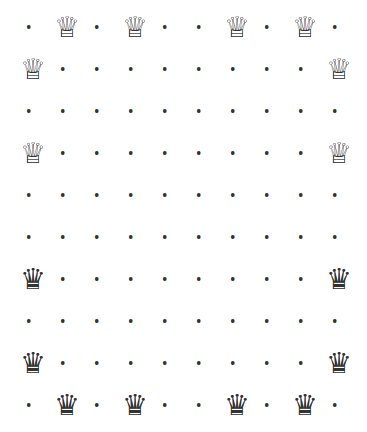
\includegraphics[scale=0.40]{log_2.png}
    \caption{Affichage de l'état initial pour un monde de taille $10\times10$.}
    \label{fig:affichage_taille_10}
\end{figure}

\section{Bibliothèque GSL}
\label{sec:gsl}

L'utilisation de ce couple (graphe, structure) permet alors de réduire une certaine complexité temporelle lors du déroulement d'une partie de jeu. 

En ce qui concerne la complexité spatiale, c'est sur le graphe encore une fois qu'il est possible d'agir pour la réduire. Chaque case possède au plus huit voisins, par conséquent dans la matrice d'adjacence représentant le graphe, au plus huit cases auront une valeur différente de 0, équivalente à la direction \texttt{NO\_DIR}. 

Alors, pour un graphe possédant $\textbf{m}$ sommets, il y aura au moins $ \textbf{m - 8}$ zéros par ligne dans la matrice. La matrice d'adjacence est donc une matrice dite creuse, c'est-à-dire contenant un grand nombre de zéros à l'intérieur.

\medbreak
Cette matrice, visible en figure \ref{subfig:graphe_normal}, est dite au format \texttt{COO} (\textit{Coordinate Storage}) et présente donc un défaut important en termes de complexité lors d'une itération sur les arêtes. \\
La bibliothèque \texttt{GSL} permet cependant de convertir cette matrice au format \texttt{CSR} (\textit{Compressed Row Format}) comme présentée en figure \ref{subfig:graphe_compresse}, ce qui permet de stocker dans un tableau seulement les valeurs non nulles de manière consécutive. La complexité lors d'itérations sur les arêtes est donc nettement améliorée.

\begin{figure}[H]
    \centering
    \begin{subfigure}{0.5\textwidth}
        \centering
        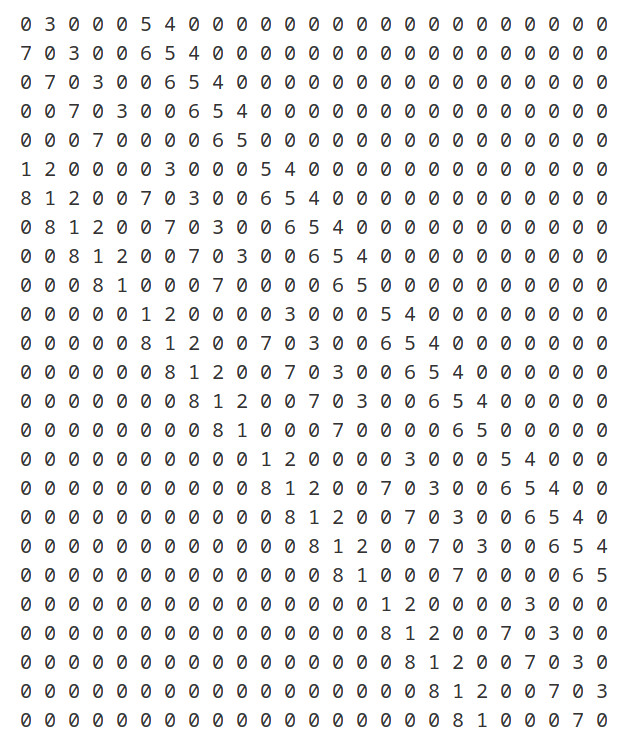
\includegraphics[scale=0.4]{graph_normal.png}
        \caption{Format COO (Coordinate Storage).}
        \label{subfig:graphe_normal}
    \end{subfigure}
    \hspace{1cm}
    \begin{subfigure}{0.4\textwidth}
        \centering
        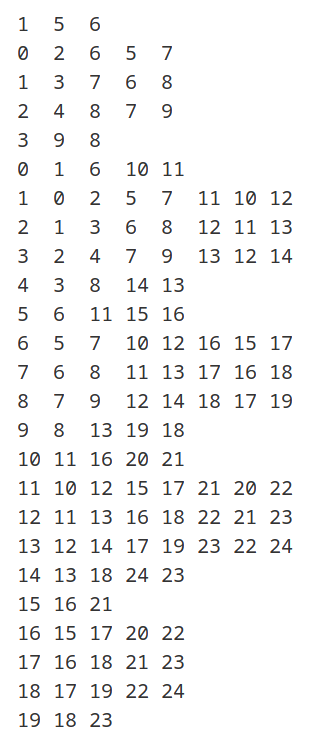
\includegraphics[scale=0.4]{graph_compress.png}
        \caption{Format CSR (Compressed Row Format).}
        \label{subfig:graphe_compresse}
    \end{subfigure}
    \caption{Matrices d'adjacence pour un monde de taille $5\times5$.\protect\footnotemark} 
    \label{fig:matrices_d_adjacence}
\end{figure} \medbreak
\footnotetext{Taille minimale d'un monde}

Ainsi, sont disponibles, un graphe de liaison statique, au sens où il n'est pas modifié durant l'exécution de la partie, auquel se référer pour des recherches plus ou moins techniques de chemin entre deux positions. Et un tableau, alloué dynamiquement, aisément manipulable, permettant un affichage simple et clair du déroulement du jeu des amazones.\\
Plusieurs autres représentations de plateaux de jeu nous ont été proposés, tel qu'un plateau en forme de donut. Ce dernier n'était pas la priorité, car le but était de faire fonctionner le jeu. Cependant, l'idée de le faire en partant d'un graphe classique, puis en condamnant uniquement les liaisons en contact avec le bord du cercle central, a commencé à être implémentée et peut peut-être piste d'amélioration future du projet.

\medbreak

Dès lors que ces aspects ont été finalisés, il a alors été possible de se lancer dans l'implémentation du jeu en lui-même. Il a fallu différencier deux côtés bien distincts, le côté serveur modifiant le monde selon l'analyse des coups reçus par le deuxième côté, le côté joueur. Cette dualité permet 